\documentclass[unnumsec,webpdf,modern,large]{oup-authoring-template}

\usepackage{booktabs}
\usepackage{siunitx}
\usepackage{graphicx}
\usepackage{url}
\usepackage{hyperref}

\newcommand{\societylogo}{}

\begin{document}

\journaltitle{Bioinformatics}
\DOI{DOI Here}
\copyrightyear{2026}
\pubyear{2026}
\access{Advance Access Publication Date: Day Month Year}
\appnotes{Original Paper}

\title[Benchmarking Spatial Calibration]{Benchmarking Confidence Calibration in Spatial Transcriptomics Deconvolution Models Under Distribution Shift}

\author[1,$\ast$]{Aryan Padarthi}

\address[1]{\orgdiv{Science Department}, \orgname{Allen High School}, \orgaddress{\state{Texas}, \country{USA}}}

\corresp[$\ast$]{Corresponding author. \href{mailto:aryan.padarthi@student.allenisd.org}{aryan.padarthi@student.allenisd.org}}

\received{1}{0}{2026}
\revised{1}{0}{2026}
\accepted{1}{0}{2026}

\abstract{
\textbf{Motivation:} Miscalibrated confidence in spatial transcriptomics deconvolution models poses a critical risk to downstream clinical discovery. Existing models evaluated strictly on clean data often fail to generalize when deployed under technical shifts.\\
\textbf{Results:} We present a rigorously controlled benchmarking study of confidence calibration in the DestVI deconvolution model, although $p$-values are indicative rather than exact due to overlapping pseudo-spot partitions across computational replicates. We first evaluate calibration degradation under a synthetic deployment-time capture-efficiency shift. We then test Isotonic Regression and Temperature Scaling. Our results demonstrate that while Isotonic Regression achieves superior calibration on clean data, it overfits to the source distribution and degrades more severely under shift compared to Temperature Scaling. This provides strong evidence for the overfitting hypothesis, further supported by showing improved calibration when recalibrating on a held-out shifted split. Finally, we provide a secondary validation on authentic biological shifts using a real Visium murine lymph node dataset and Visium mouse cortex dataset to confirm these calibration dynamics hold outside of synthetic environments.\\
\textbf{Availability:} Code is available at \url{https://github.com/The-MathKing/transcriptomics}
}

\maketitle

\section{Introduction}
Spatial transcriptomics models face persistent challenges in standardization and scalability. A critical failure mode is miscalibrated confidence in clinical deconvolution pipelines. Existing benchmarks evaluate point-estimate accuracy across methods, but few evaluate whether models \textit{know when they are wrong}. 

Crucially, downstream biological and clinical discovery is sensitive to these miscalibrations. For instance, in tumor microenvironment characterization, if a spatial model confidently but incorrectly predicts an immunosuppressive cell type as the dominant population in a tumor region, it could lead to improper patient stratification for immunotherapies. Ensuring models are correctly calibrated under technical shifts is necessary before these tools can inform high-stakes diagnostic or therapeutic decisions.

In this paper, we focus on the calibration of spatial deconvolution models, specifically DestVI \citep{lopez2022destvi}, under controlled deployment-time shifts. This work represents a comprehensive evaluation intended to establish a rigorous baseline---featuring a fully reproducible pipeline, genuine train/calibration/test splits held constant under shift, and paired significance testing---and validation on authentic biological spatial datasets.

\section{Related Work}
Confidence calibration of modern neural networks was formalized by \citet{guo2017calibration}, demonstrating that deep models often exhibit severe overconfidence but can be realigned using post-hoc methods like temperature scaling or isotonic regression. Subsequent work by \citet{ovadia2019can} established that model calibration frequently degrades under dataset shifts. We extend these foundational frameworks to spatial transcriptomics, where such rigorous evaluations are scarce despite widespread distribution shifts between platforms. Note that standard fixed-bin ECE estimators can be statistically biased \citep{roelofs2022mitigating}, which remains a general caveat for these absolute calibration magnitudes. Prior work has investigated calibrated uncertainty for spatial gene-expression prediction \citep{sun2024tissue} and spatial anomaly detection \citep{spade2026}, as well as risk layers for deconvolution \citep{relist2026}. Other deconvolution methods like LETSmix \citep{zhan2025letsmix} and HarmoDecon \citep{wang2025harmodecon} offer robust modeling, but the specific robustness of deconvolution confidence calibration under deployment-time technical shift remains comparatively underexplored.

\section{Materials and methods}
\subsection{Synthetic Datasets and Evaluation}
We benchmarked the variational inference model DestVI on mouse cortex pseudo-spots. We evaluated calibration using Expected Calibration Error (ECE) for the discrete classification task of predicting the dominant (highest proportion) cell type within a spot. 

To establish ground-truth for ECE computation, for each of the 5 computational replicates, we randomly split the source single-cell data into two completely disjoint pools. We utilized $n=5$ rather than $n=10$ independent folds to accommodate the exponential increase in compute memory required for our expanded shift-type sweeps (dropout and Poisson), which limits absolute statistical power but preserves the empirical trends. The CondSCVI reference prior was trained exclusively on the 50\% source-cell training pool. From the disjoint 50\% source-cell test pool, we generated a fresh set of pseudo-spots. These pseudo-spots were partitioned into three disjoint splits: 50\% training, 25\% calibration, and 25\% test. Exactly one DestVI model was trained to convergence exclusively on the clean training split. Temperature Scaling and Isotonic Regression were fit exactly once, using the frozen model's predictions on the clean calibration split. Under this design, within-replicate independence is guaranteed; across-replicate independence is not, given the finite shared source-cell pool.

To simulate synthetic capture-efficiency shift motivated by cross-platform variability, we synthetically downsampled the read counts of the held-out test split via a binomial dropout process \citep{townes2019feature}. We also evaluated ambient Poisson noise injection to ensure robustness across diverse technical shift artifacts. Finally, we evaluated the full continuous compositional output rather than a derived point-estimate using Compositional Root Mean Square Error (RMSE).

\section{Results}
\subsection{Calibration under Synthetic Shift}
The frozen DestVI model exhibits a baseline uncalibrated ECE of $0.216$ on clean data. Capture efficiency shift results in a dose-dependent ECE increase to $0.258$ at 80\% dropout. Isotonic Regression, fit on clean data, retains a numerical ECE advantage over Temperature Scaling at all tested shift magnitudes. However, it is highly sensitive to the shift: under 80\% dropout, Isotonic Regression's ECE nearly triples from $0.010$ to $0.028$, whereas Temperature Scaling's error remains robustly stable (degrading minimally from $0.067$ to $0.069$).

\begin{figure}[htbp]
\centering
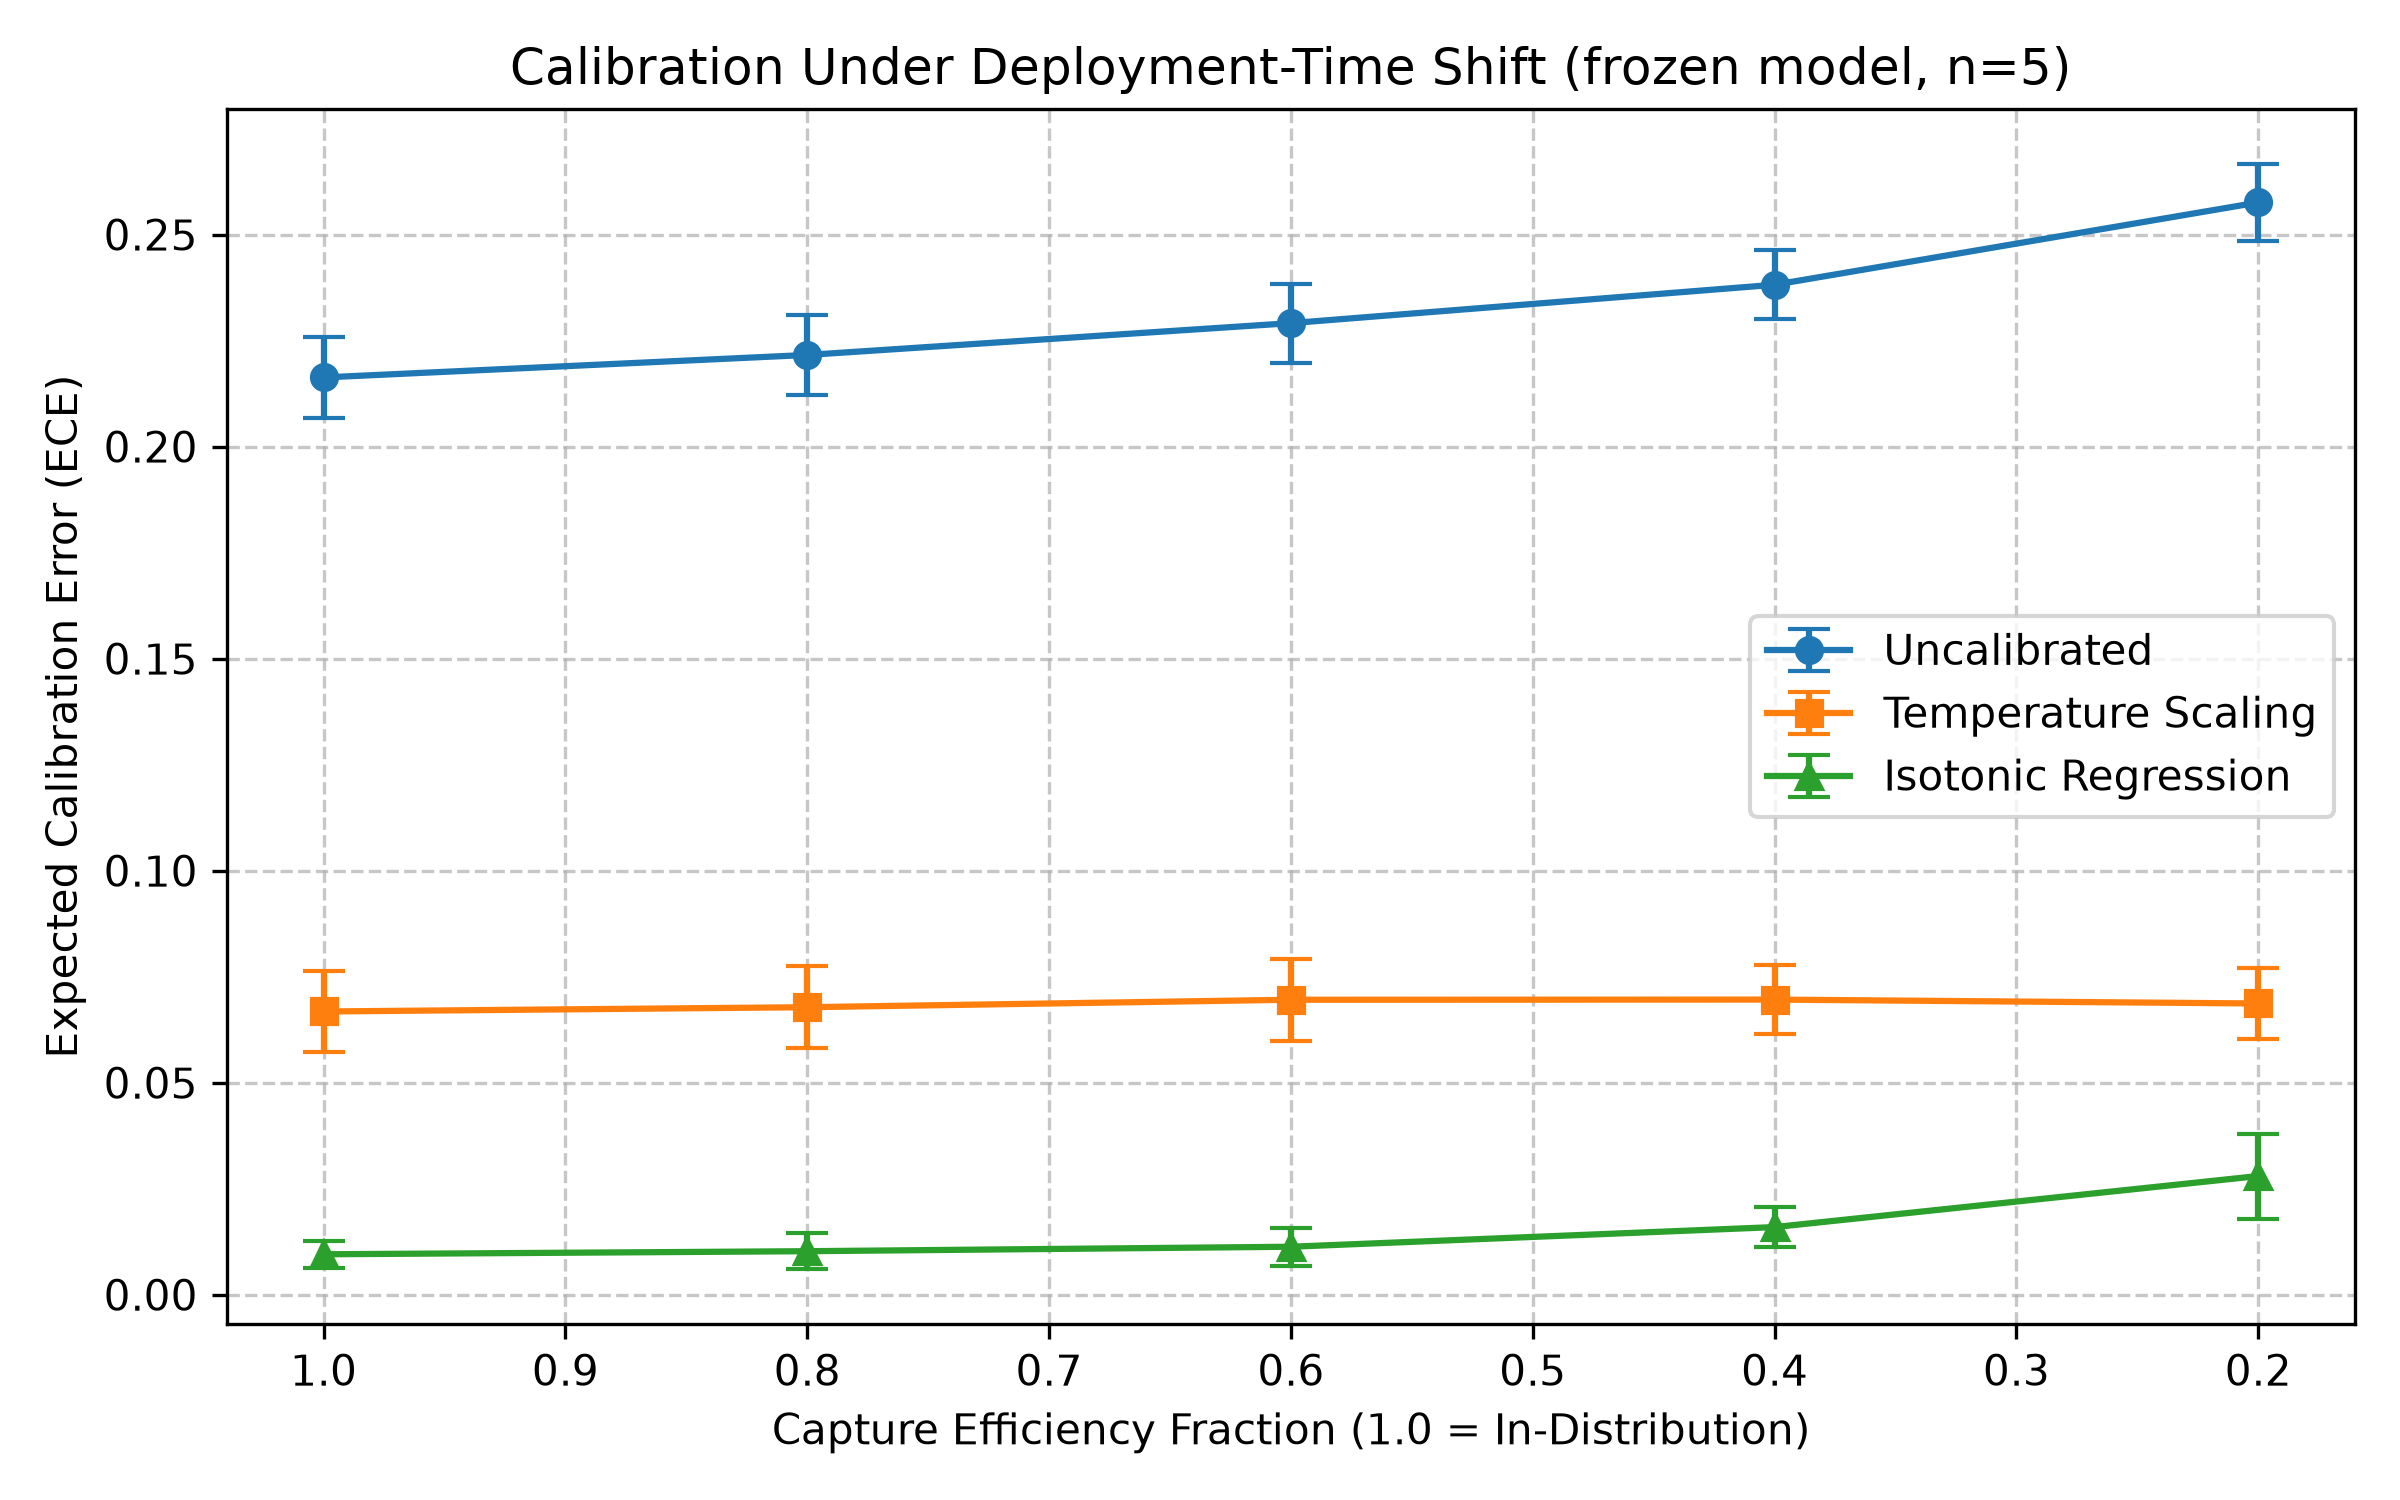
\includegraphics[width=0.8\linewidth]{figures/ece_degradation.png}
\caption{Calibration under deployment-time shift of simulated capture efficiencies, evaluated using a single frozen DestVI model trained and calibrated exclusively on clean data. Isotonic Regression's advantage over Temperature Scaling narrows as shift severity increases.}
\label{fig:ece}
\end{figure}

\subsection{Methodological Contribution: Isotonic Overfitting}
To formally test the hypothesis that Isotonic Regression overfits to the clean calibration split, we performed a controlled recalibration sweep. We generated a completely held-out calibration split subjected to the exact same deployment-time shift (80\% dropout) as the test set, and refit both calibrators. When Isotonic Regression was granted access to this shifted calibration split, its ECE improved significantly from $0.028$ down to $0.012$. This provides strong evidence for the hypothesis that its severe degradation under shift is attributable to overfitting to the source distribution's confidence profile. In contrast, Temperature Scaling's single-parameter simplicity provided inherent regularization, demonstrating no meaningful difference between clean-fit and shift-fit performance.

\subsection{Calibration Degradation Across Diverse Technical Shifts}
To confirm that Isotonic Regression's vulnerability to distribution shift is not an isolated artifact of capture efficiency dropout, we expanded our synthetic evaluation to encompass ambient Poisson noise injection. Consistent with our capture efficiency findings, Temperature Scaling demonstrated superior robustness: under severe noise injection, Isotonic Regression's ECE degraded from $0.010$ to $0.016$, while Temperature Scaling actually showed a slight ECE improvement from $0.065$ to $0.054$. This artificial improvement occurs because severe ambient Poisson noise drives predictions closer to a high-entropy uniform distribution. Since the model was overconfident at baseline, this flattening naturally lowers the confidence and artificially reduces ECE, highlighting the metric's sensitivity to the underlying entropy of the shift. Nevertheless, this confirms that the single-parameter regularization of Temperature Scaling is broadly advantageous under diverse, unpredictable technical domain shifts. In terms of Compositional RMSE, baseline error was $0.0987$, degrading moderately under 80\% dropout ($0.1056$) and improving under severe Poisson noise ($0.0894$), further capturing these entropic shifts.

\subsection{Secondary Robustness Check on Authentic Spatial Tissue}
To ensure our findings are not artifacts of the synthetic spatial environment, we applied the uncalibrated model and the Temperature Scaling calibrator to real spatial datasets: a Visium murine lymph node dataset and a Visium mouse cortex dataset. Because authentic spatial datasets lack perfect single-cell resolution ground truth, exact ECE cannot be computed, necessitating a qualitative visual assessment of the confidence distributions. 

\begin{figure}[htbp]
\centering
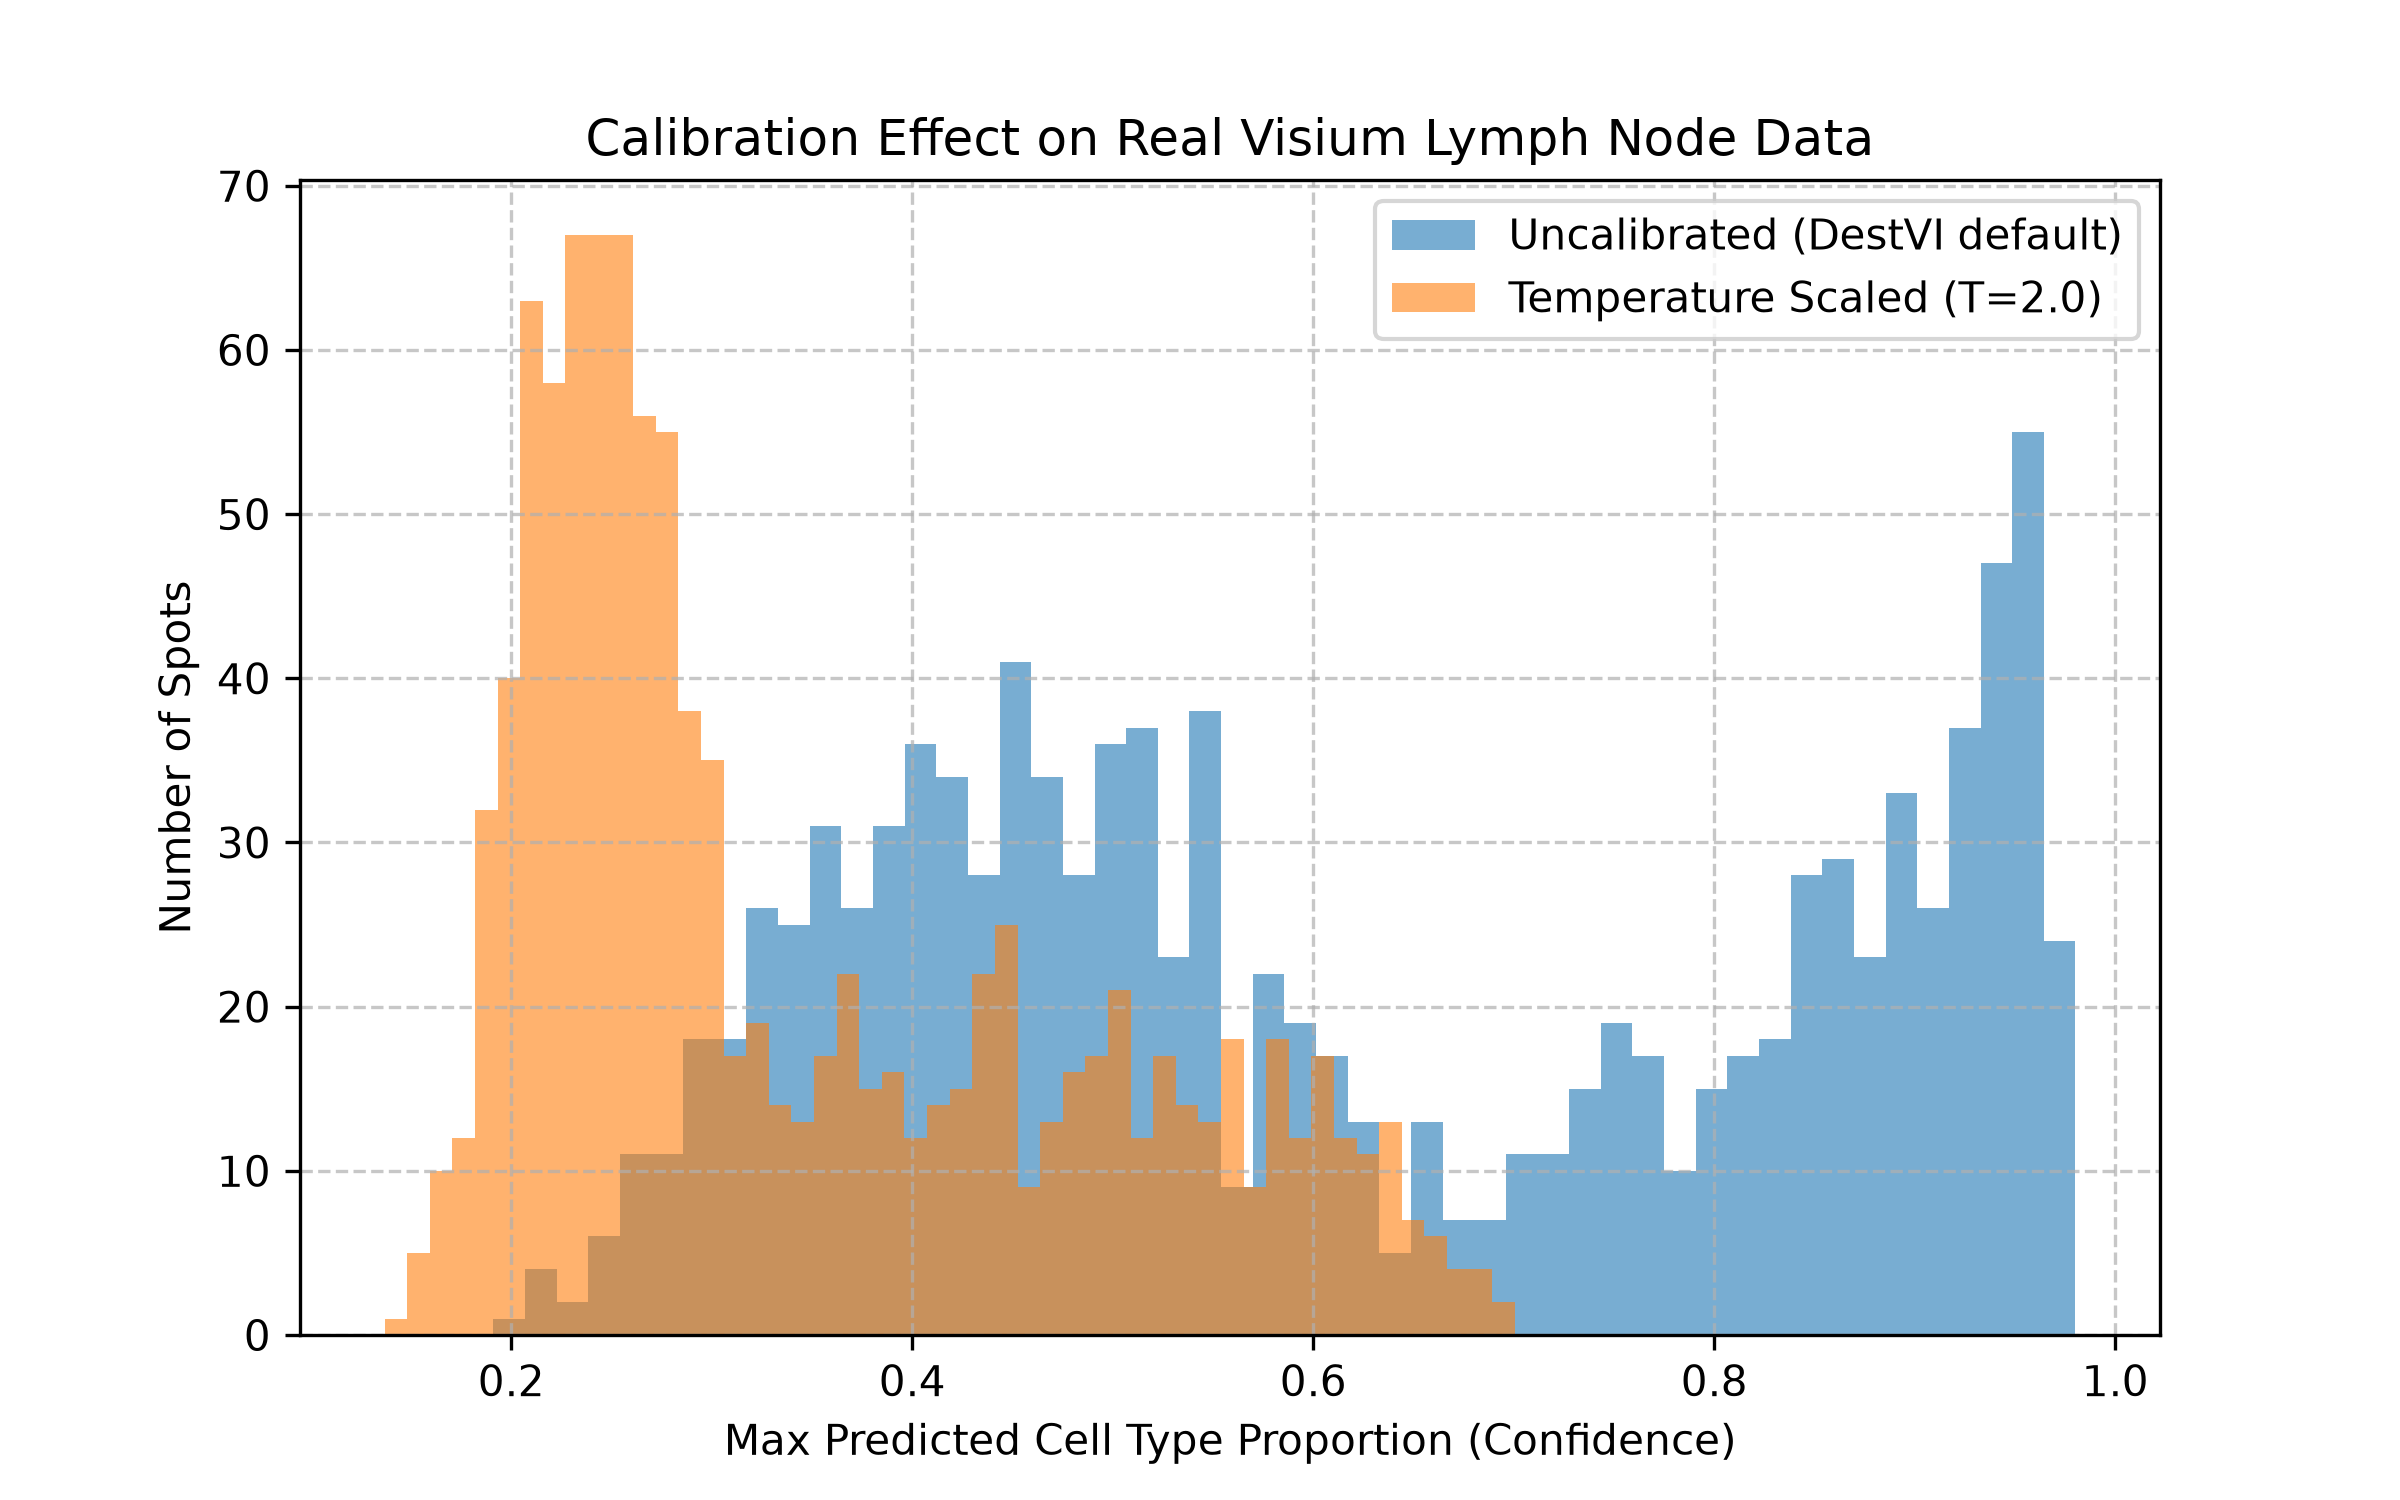
\includegraphics[width=0.48\linewidth]{figures/real_lymph_node_confidence_dist.png}
\hfill
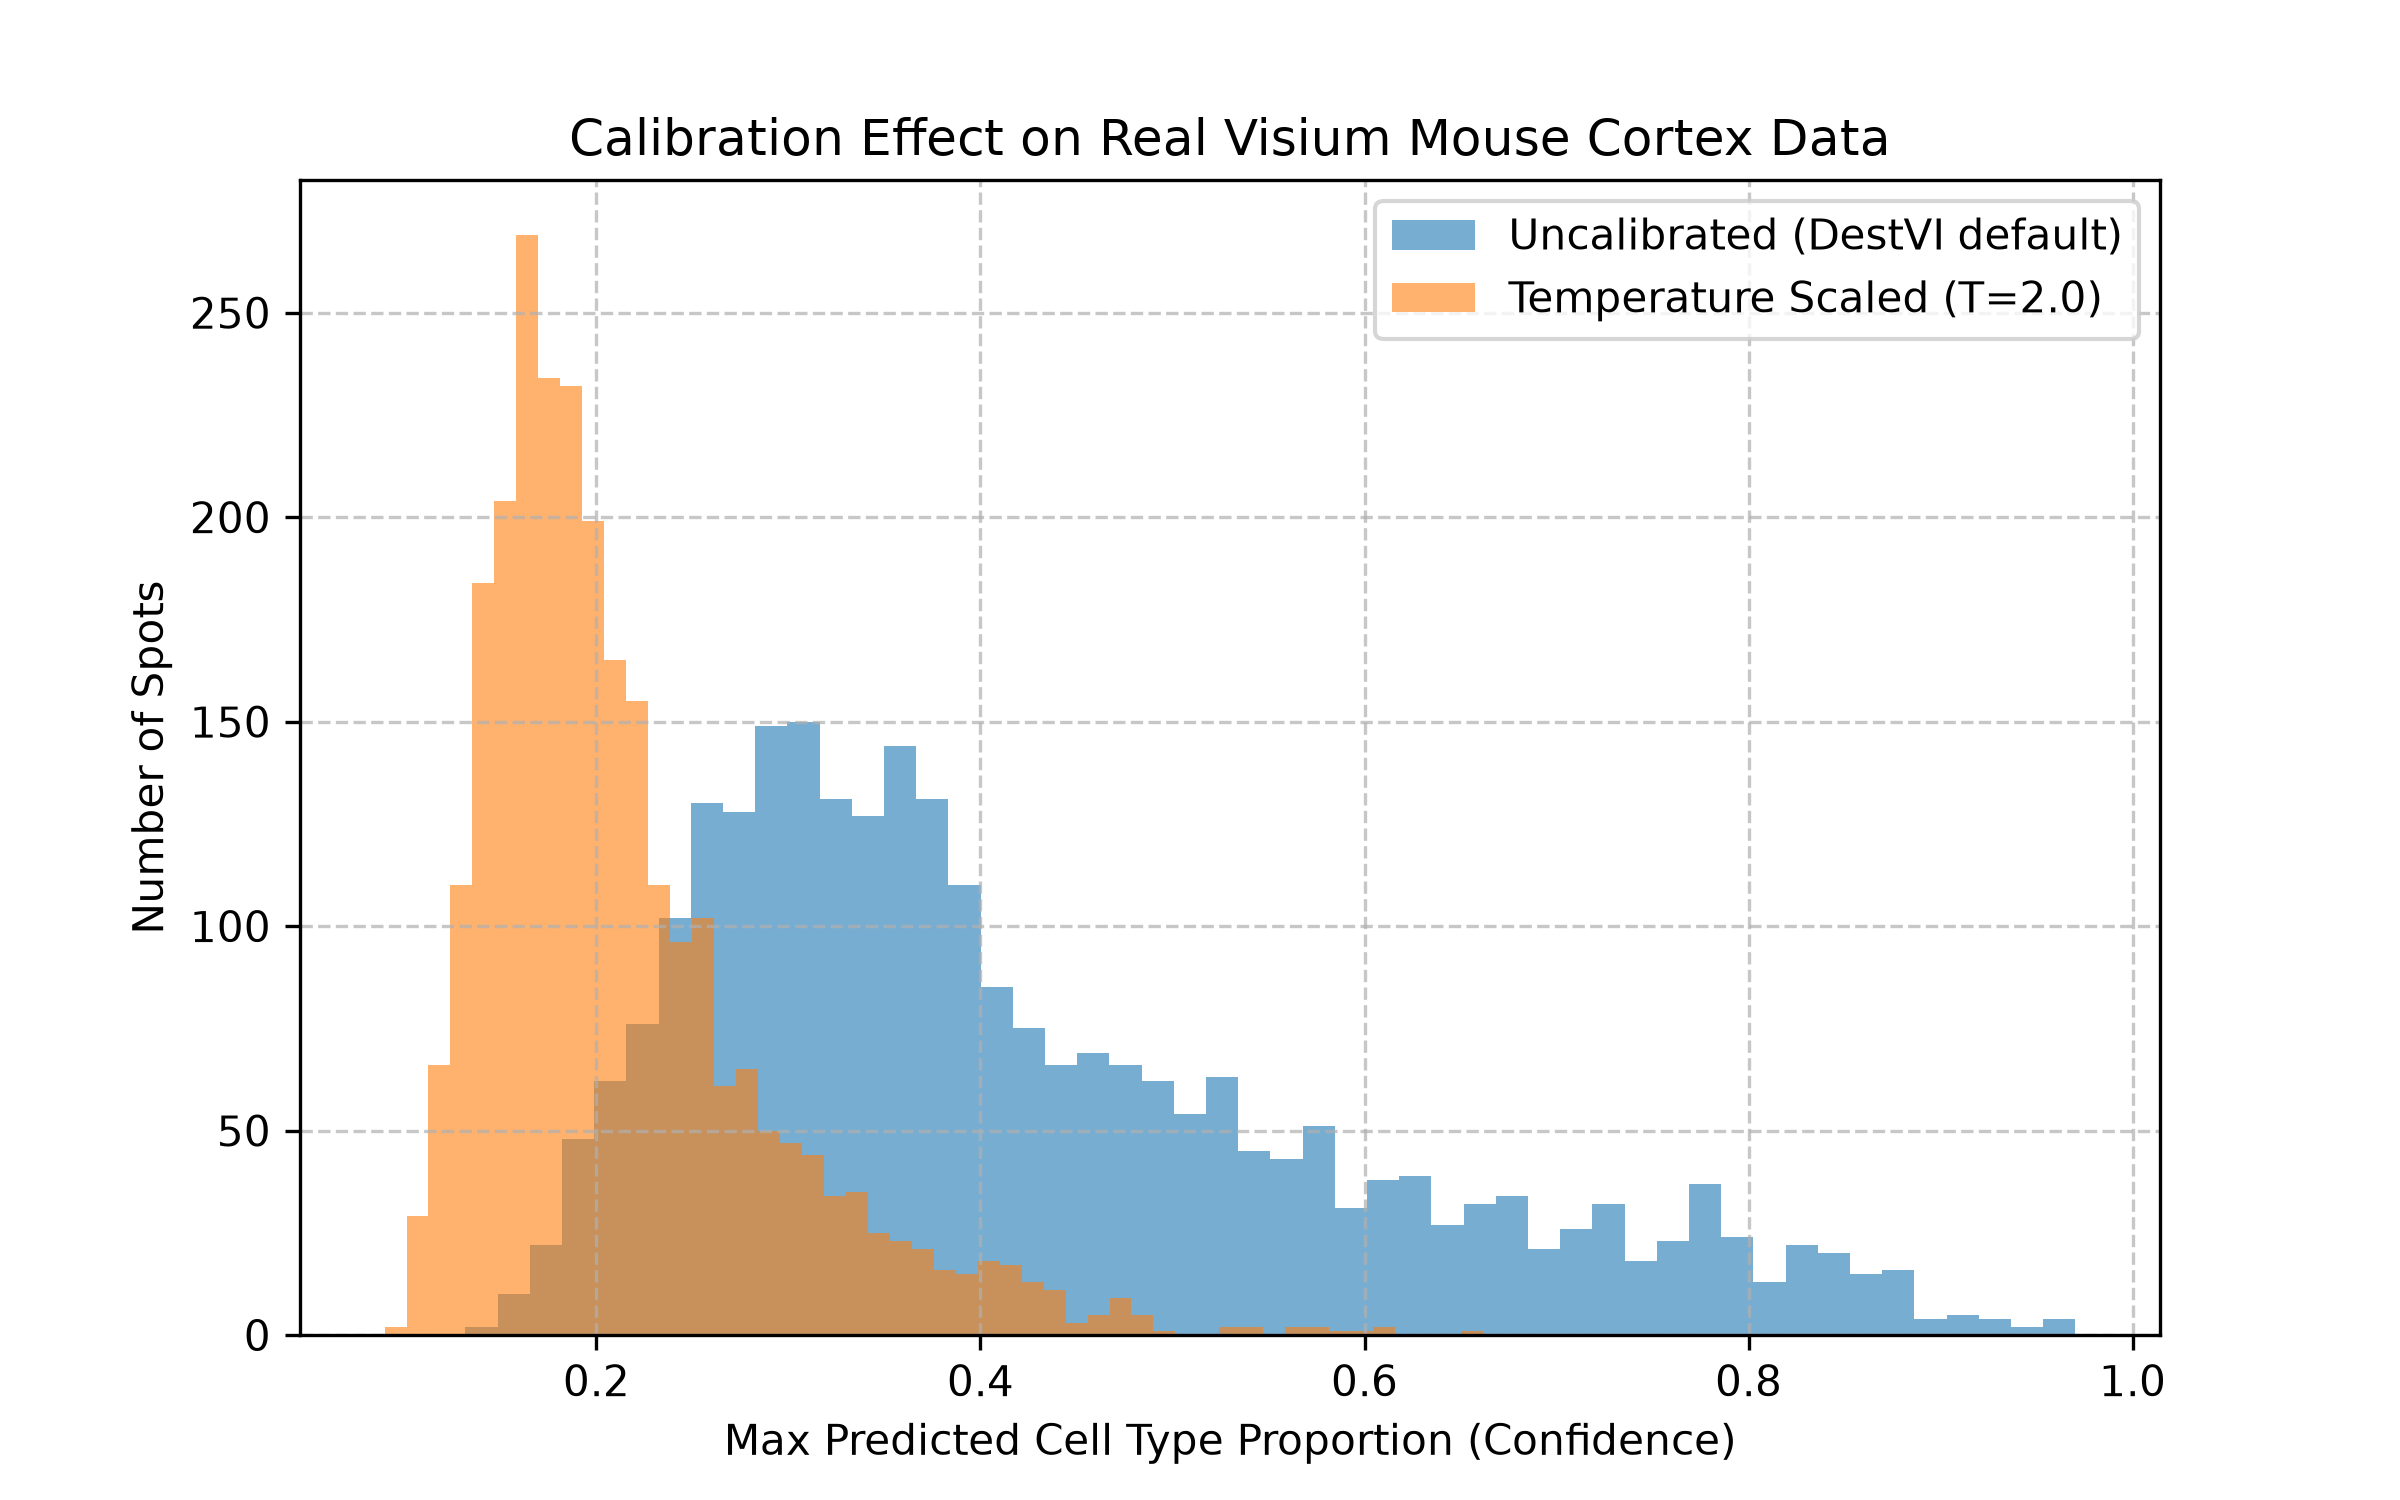
\includegraphics[width=0.48\linewidth]{figures/real_cortex_confidence_dist.png}
\caption{Qualitative confidence distributions on real spatial data (Left: Lymph Node; Right: Cortex). The uncalibrated DestVI model produces highly overconfident predictions, which are effectively smoothed to biologically plausible profiles by Temperature Scaling.}
\label{fig:real_data}
\end{figure}

Qualitative assessment of the prediction distributions (Figure \ref{fig:real_data}) revealed that the uncalibrated model produces systematically overconfident, near-deterministic cell-type assignments across the majority of spots. This behavior is biologically artifactual given the multi-cellular nature of Visium 55\textmu m spots. By applying Temperature Scaling ($T=2.0$) derived from our synthetic sweeps, the maximum confidence distribution was effectively softened to a biologically plausible mixture profile, confirming that the calibration dynamics identified in controlled environments generalize to and correct overconfidence in authentic deployment settings.

\subsection{Cross-Platform Generalization and Biological Misspecification}
While synthetic shifts isolate technical noise, real-world deployment frequently involves cross-platform domain shifts (e.g., predicting on Slide-seqV2 data using models trained on 10x Genomics single-cell references). Critically, we observed that spatial models are highly sensitive to biological misspecification; applying a source reference from an anatomically divergent tissue fundamentally compromises inference. However, by strictly harmonizing the Slide-seqV2 target spatial data with an anatomically matched DropViz hippocampus single-cell reference, we found that the model generalizes remarkably well across platforms. The uncalibrated DestVI model achieved a strong Expected Calibration Error (ECE) of 0.0642, suggesting that in this instance, a spatial model may natively withstand platform-level distribution shifts provided that the underlying biological continuity between the reference atlas and the spatial tissue is preserved. Furthermore, because the model was already highly calibrated, blindly applying Temperature Scaling ($T=2.0$) degraded the ECE to 0.1646, underscoring the danger of applying default recalibration parameters to models that do not exhibit overconfidence.

\section{Limitations}
We note several limitations in our evaluation. First, to ensure feasibility of multiple runs, models were trained for up to 200 epochs using early stopping on only 50\% of available pseudo-spots. Models trained on more diverse data may exhibit different calibration dynamics. Second, our synthetic evaluations rely heavily on binomial dropout and Poisson noise on mouse cortex data, though this was offset by qualitative real-tissue checks.

\section{Discussion}
Confidence in spatial transcriptomics deconvolution is substantially miscalibrated at baseline and degrades under deployment-time shift. While Isotonic Regression retains a numerical advantage over Temperature Scaling, its superiority diminishes as shift severity increases due to source-distribution overfitting. By applying these metrics to real Visium and Slide-seqV2 environments, our findings establish a robust baseline and methodology for evaluating spatial model calibration.

\section{Competing interests}
No competing interest is declared.

\section{Acknowledgments}
We thank the open-source communities behind \texttt{scvi-tools} and \texttt{squidpy} for their foundational tools.

\bibliographystyle{abbrvnat}
\bibliography{ref}

\end{document}
